\documentclass[12pt, letterpaper]{article}
\usepackage{amsmath}
\usepackage{amssymb}
\usepackage{graphicx} 
\title{STA 629 - Homework 1}
\author{Anthony Bernardi}
\date{September 16, 2024}
\begin{document}
\maketitle

\section{Problem 1} 

This answer covers problem 3.6 from the book. 

Show that the ridge regression estimate is the mean and mode of the posterior distribution of $\beta$ under a Gaussian prior and a Gaussian sampling model. Find the relationship between the regularization parameter $\lambda$ and the variances $\tau$ and $\sigma^2$. 

We begin by noting the following. The prior is distributed as such $\beta \sim N(0, \tau I)$ and the likelihood is distributed as such $y \sim N(X\beta, \sigma^2I)$.

We will approach this problem by writing out Bayes' Theorem. 

\[
p(\beta | y) = \frac{p(y | \beta) p(\beta)}{p(y)}
\]

Which can be thought of in the following way. 

\[
\text{posterior} = \frac{N(X\beta, \sigma^2 I) \cdot N(0, \tau I)}{P(Y)}
\] 

Noting that the denominator is a constant, we can write the numerator as such with respect to the multivariate normal. 

\[
exp(-\frac{1}{2} (y - X\beta)^T \frac{1}{\sigma^{-2}} (y - X\beta) - \frac{1}{2} \beta^T \frac{1}{\tau} \beta)
\]

We can simplify this expression by expanding the terms. 

Now for convenience, we can take the log of both sides of the posterior expression, which simplifies to the following.  

\[
\text{log posterior} = -\frac{1}{2} (y - X\beta)^T \frac{1}{\sigma^{-2}} (y - X\beta) - \frac{1}{2} \beta^T \frac{1}{\tau} \beta
\]

We can now consider a way to make this equivalent to our ridge regression estimate. Let $\lambda = \frac{\sigma^2}{\tau}$, and this gives us the following. 

\[
-\frac{1}{2} \cdot \frac{1}{\tau} (Y - X\beta)^T (Y - X\beta) + \frac{\sigma^2}{\tau^2} \beta^T \beta
\]

Which we can see, this is equivalent to the ridge regression estimate.

\section{Problem 2} 

We will download the provided microarray data provided from Canvas. This is from a gene expression study with $n = 83$ observations and $p = 2308$ genes, including the response variable $y$. 

\subsection{Part a}

Fit the models and visualize regularization paths for each of the following model frameworks. 

\begin{itemize}
\item Lasso 
\item Elastic Net 
\item SCAD
\item MCP
\end{itemize}

We will start by including our Python code, used to build and fit the Lasso and Elastic Net models, as well as including the plots of their regularization paths. 

\begin{verbatim} 
import pandas as pd 
import numpy as np 
import matplotlib.pyplot as plt 
from sklearn import linear_model 

X = pd.read_csv("/home/adbucks/Documents/sta_629/Homework_1/X_SRBCT.csv", header = None)
y = pd.read_csv("/home/adbucks/Documents/sta_629/Homework_1/Y_SRBCT.csv", header = None)

# looks okay, so we can convert the response variable to numpy array to be sure 

y = y.to_numpy() 
y = y.flatten()

# now the modeling 
from sklearn.linear_model import ElasticNet, Lasso, enet_path, lasso_path 

e_model = ElasticNet(random_state = 1870)

e_model.fit(X, y)

# now the lasso model 
lasso_m = linear_model.Lasso()
lasso_m.fit(X, y)

# now we can try to do the plotting 
eps = 5e-3  
alphas_e, coefs_e, _ = enet_path(X, y, eps = eps) 

# now the lasso path 
alphas_l, coefs_l, _ = lasso_path(X, y, eps = eps)

# now we can try to do a quick print check 
print("Gut check 1...") 
print(alphas_e.shape, coefs_e.shape)
print("Gut check 2...")
print(alphas_l.shape, coefs_l.shape)

# have to transpose the coefficients before plotting 
coefs_et = np.transpose(coefs_e)
coefs_lt = np.transpose(coefs_l)
print("Gut check 3...")
print(coefs_et.shape, coefs_lt.shape) 

plt.plot(alphas_e, coefs_et)
plt.xlabel("alpha") 
plt.ylabel("coefficients") 
ymin, ymax = plt.ylim()
plt.title("Elastic Net Regularization Path") 
plt.axis('tight')
plt.show() 

# this seems to work now! we can go through the lasso path now 
plt.plot(alphas_l, coefs_lt)
plt.xlabel("alpha")
plt.ylabel("coefficients")
ymin, ymax = plt.ylim() 
plt.title("Lasso Regularization Path") 
plt.axis('tight') 
plt.show() 

# Now done with the plotting, we will try and get a sense of the most important variables, and try to get a sense of how the models compare 
# we can start with scoring 

print("Elastic Net Score: ", e_model.score(X, y)) # 0.306
print("Lasso Score: ", lasso_m.score(X, y)) # 0.103 

# seems like the elastic net model is better than the lasso model in terms of R squared values 
# we can try and get a sense of the most important variables now 

coefs_e = e_model.coef_ 
coefs_l = lasso_m.coef_

print("Coefficients gut check...")
print(type(coefs_e), type(coefs_l))

# want to sort the absolute value of the coefficients 
coefs_e = np.abs(coefs_e) 
coefs_l = np.abs(coefs_l) 

coefs_e = np.sort(coefs_e)[::-1] # reverse order workaround 
coefs_l = np.sort(coefs_l)[::-1] 

print("Elastic Net Coefficients: ", coefs_e) 
print("Lasso Coefficients: ", coefs_l) 

# per the homework, we can pull out the top 10 variables 

top_10_enet = coefs_e[0:10] 
top_10_lasso = coefs_l[0:10] 

print("Top 10 Elastic Net Coefficients: ", top_10_enet) 
print("Top 10 Lasso Coefficients: ", top_10_lasso) 

# trying it another way 
coefs = lasso_m.coef_  

non_zero = [i for i, coef in enumerate(coefs) if coef != 0]

# now trying to find the feature names 
non_zero_feature_names = [X.columns[i] for i in non_zero]
non_zero_values = [coefs[i] for i in non_zero]

# trying to print the results 
for name, value in zip(non_zero_feature_names, non_zero_values):
    print(f'Feature: {name}, Coefficient: {value}')

# I think this makes sense, and we can try to do the same for the elastic net now 
coefs_e = e_model.coef_

non_zero_e = [i for i, coef in enumerate(coefs_e) if coef != 0]

non_zero_feature_names_e = [X.columns[i] for i in non_zero_e]
non_zero_values_e = [coefs_e[i] for i in non_zero_e]

# now trying to fancy print 
for name, value in zip(non_zero_feature_names_e, non_zero_values_e):
    print(f'Feature: {name}, Coefficient: {value}')

\end{verbatim}

We will include the regularization plots for the Elastic Net and Lasso Models here now. 

\begin{figure} 
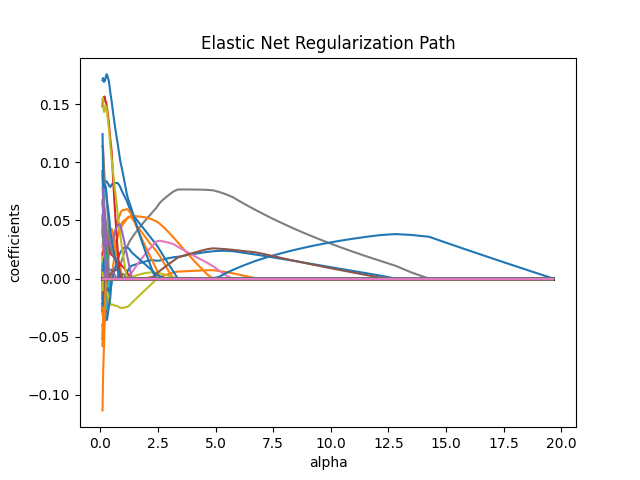
\includegraphics{/home/adbucks/Documents/sta_629/Elastic_Net_Reg_Path.png} 
\caption{Elastic Net Regularization Path} 
\end{figure} 

\begin{figure}
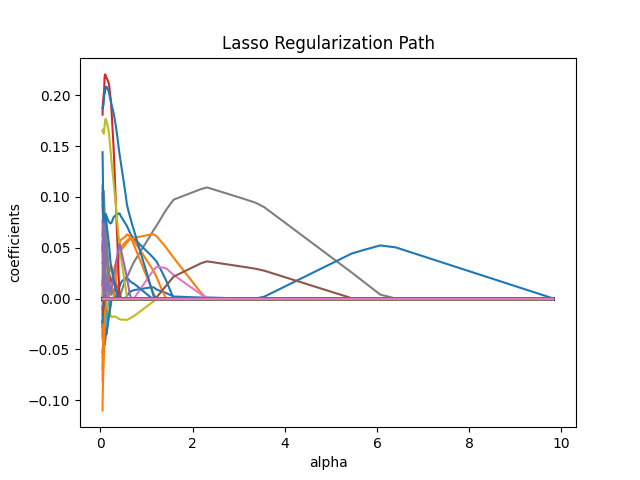
\includegraphics{/home/adbucks/Documents/sta_629/Lasso_Reg_Path.png} 
\caption{Lasso Regularization Path} 
\end{figure} 


The above Python code allows us to fit, plot, and score both the Lasso and Elastic Net models. We can see that the Elastic Net model has a higher $R^2$ value than the Lasso model
, which we will talk about in part b. 

The R code for the SCAD and MCP models is as follows. 

\begin{verbatim} 
# loading the necessary libraries 
library("grpreg")
library("lars")
library("ncvreg")

# loading the data 
X <- read.csv("/home/adbucks/Documents/sta_629/Homework_1/X_SRBCT.csv", header = FALSE)
y <- read.csv("/home/adbucks/Documents/sta_629/Homework_1/Y_SRBCT.csv", header = FALSE) 
head(X)
dim(X)
dim(y)

# comparing 
class(X) # need to convert to matrix array 
X <- as.matrix(X)

class(y) # need to convert to numeric
y <- y V1 # normally the dollar operator would be used, but not for the latex document 


# now we can do the actual modeling with the data loaded and get to plotting
# and eventually scoring 
# using another package to avoid the grouped covariates problem 
# need to coerce y into a numeric 
# trying another way 

mc_model2 <- ncvreg(X, y) # MCP default 
# maybe we're having the transpose problem again

plot(mc_model2, type = "scale", vertical.line = TRUE)

summary(mc_model2)

# it appears we have many 0 coefficients and a sparse model, which, when 
# selecting specific alpha, allows us to see which variables are most 
# strongly correlated with the outcome variable

# we can now try this with the SCAD penalty to observe any differences
mc_model_scad <- ncvreg(X, y, penalty = "SCAD")

# can now observe any differences 
plot(mc_model_scad, type = "scale")

summary(mc_model_scad)

# we can try cross-validating to get around the lambda issue 
cvfit <- cv.ncvreg(X, y)
summary(cvfit)

cvfit_scad <- cv.ncvreg(X, y, penalty = "SCAD")
summary(cvfit_scad)
\end{verbatim}

The above R code allows us to fit, plot, and score both the SCAD and MCP models.
We can see that the SCAD model has a higher $R^2$ value than the MCP model, which we will talk about in part b. 

We will now include the regularization plots for the MCP and SCAD models here. 

\begin{figure}
  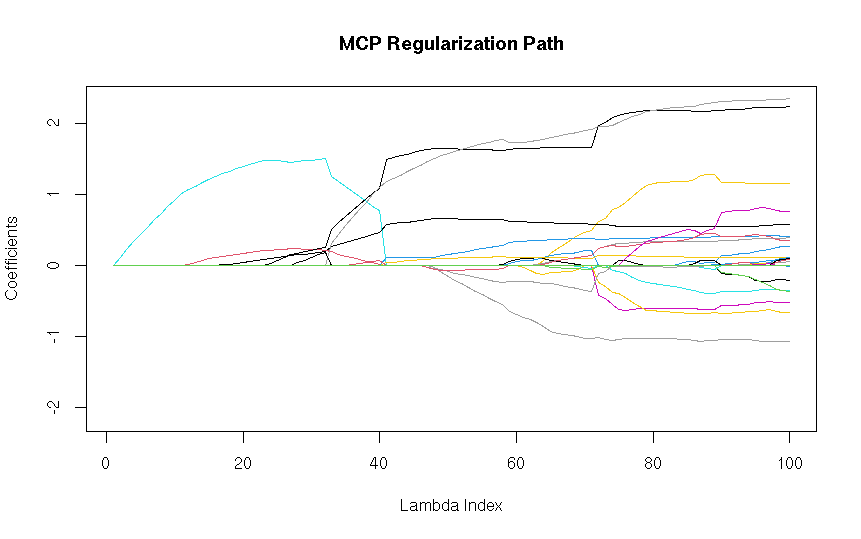
\includegraphics[width=\textwidth]{/home/adbucks/Documents/sta_629/Homework_1/MCP Regularization Path Plot.png}
  \caption{MCP Regularization Path}
\end{figure}


\begin{figure}
  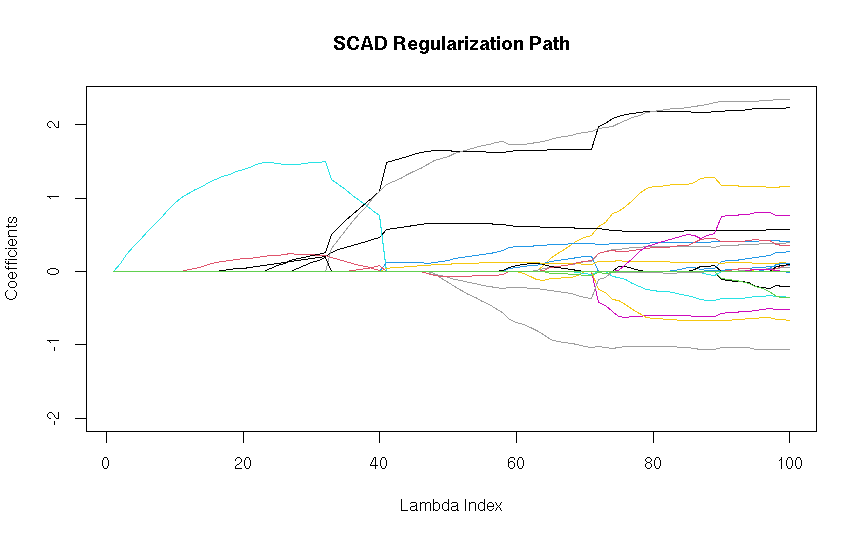
\includegraphics[width=\textwidth]{/home/adbucks/Documents/sta_629/Homework_1/SCAD Regularization Path Plot.png}
  \caption{SCAD Regularization Path}
\end{figure} 

\subsection{Part b} 

Interpret the results. What are the top genes selected by each method? Are they different? If so, why? Which regularization paths look the most variable? Why is this the case? If you had to report 
the genes of interest to a scientist, which would you choose and why? 

The top genes selected by each method are as follows. For the elastic net model, with a $R^2$ value of 0.306, there were 7 top genes with non-zero coefficients selected, and they included records 150, 271, 330, 467, 508, and 1930. It should be noted that the two largest coefficient values were 1930 and 150. 

For the lasso model, with a $R^2$ value of 0.103, there were 2 top genes with non-zero coefficients selected, and they included records 150 and 508. It should be noted that the larger coefficient in terms of absolute value was 508, and the second largest was 150. 

Per the R output, the SCAD model had a $R^2$ value of 0.44, and featured 24 non-zero coefficients. The top genes and features in this case were records 849, 844, 473, 1240, 1592, 111, 244, 271, 372, and 441. The largest coefficients in this case were 1240 and 849. 

Finally, the MCP, or MC+ model had a $R^2$ value of 0.27, and featured 8 non-zero coefficients. The top genes and features in this case were records 849, 473, 1240, 844, 1319, 1592, 2104, and 2106, with 849 and 1240 being the largest cofficients. 

The regularization paths that look the most variable are the SCAD and MCP models. This is because they have the highest $R^2$ values, and the most non-zero coefficients. This is likely due to the fact that the SCAD and MCP models are more flexible than the Lasso and Elastic Net models, and can handle more complex data in a broad sense. 

As to the variables selected, there is quite a difference in the features selected, and eventually the non-zero coefficients for each of the models, with some overlap. As to why that is, I would posit that the shrinkage methods are quite different, and the differing algorithms results in different feature selection methods and coefficient methods. Clearly, despite the common data generating process, the observed R-Squared methods are quite different for all models. 

Genes 150 and 508 show up in a non-zero manner in multiple models, while genes 1930 and 271 show up in the Elastic Net and SCAD models. If I had to report the genes of interest to a scientist, I would choose genes 150 and 508, as they show up in multiple models, and are likely to be the most important in terms of predicting the outcome variable. Additionally, the coefficients are largest in the SCAD model for genes 1240 and 849, and they are orders of magnitude larger than those in the Lasso and Elastic Net models, so I believe this bears mentioning. Finally, I would suggest to the consulting scientist genes 473 and 1292, as these show up in the model with the highest $R^2$ value, the SCAD model. 

































\end{document}
